\documentclass[11pt,letterpaper]{article}
\usepackage[lmargin=1in,rmargin=1in,tmargin=1in,bmargin=1in]{geometry}
\usepackage{../style/homework}
\usepackage{../style/commands}
\setbool{quotetype}{false} % True: Side; False: Under
\setbool{hideans}{false} % Student: True; Instructor: False

% Plot Open/Closed Circles
\pgfplotsset{soldot/.style={color=black,only marks,mark=*},
		holdot/.style={color=black,fill=white,only marks,mark=*},
		compat=1.12
}

% -------------------
% Content
% -------------------
\begin{document}

\homework{8: Due 10/12}{The study of Mathematics, like the Nile, begins in minuteness but ends in magnificence.}{Charles Caleb Colton}

% Problem 1
\problem{10} Let $A= \{ 2, 6, 8, 10 \}$, $B$ be the set of nonnegative even numbers that are at most 10, and $C$ be the set of perfect squares less than 10. Define $f: A \to \mathbb{Z}$ and $g: B \setminus C \to \mathbb{Z}$ via $x \to \frac{15(x + 8)}{x}$ and $x \mapsto \frac{5(x^2 - 16x + 88)}{4}$, respectfully. Fully justifying your answer, determine whether $f \equiv g$. \pspace

\sol To show that two functions $f, g$ are equal, i.e. $f = g$ or $f \equiv g$, we need to show that they have the same domain, the same codomain, and their outputs are the same everywhere on their `common domain.'\footnote{Note: This is not the same as the two functions having the same image. For example, take $A= \{ 1, 2 \}$ and $B= \{ a, b \}$. Define $f, g: A \to B$ via $f(1)= a$, $f(2)= b$, and $g(1)= b$ and $g(2)= a$. Clearly, $f, g$ have the same domain and codomains. The image of both $f$ and $g$ are the same---namely, the set $\{ a, b \}$, but observe $a= f(1) \neq g(1)= b$ and $b= f(2) \neq g(2)= a$.} \pspace

{\itshape Equal Domains, $A= B$:} We need to show $A= B$ that is, we need to show that $A$ and $B$ have all the same elements. We know that $A= \{ 2, 6, 8, 10 \}$. Now $B$ is the set of nonnegative even numbers less than 10, i.e. $B= \{ 0, 2, 4, 6, 8, 10 \}$. Furthermore, $C$ is the set of perfect squares less than 10, i.e. $C= \{ 0, 4, 9 \}$. But then $B \setminus C= \{ 2, 6, 8, 10 \}$. Therefore, $A= B \setminus C$. \pspace

{\itshape Equal Codomains, $\mathbb{Z}= \mathbb{Z}$:} It is immediately clear that $f$ and $g$ have the same codomain---namely, $\mathbb{Z}$. \pspace

{\itshape Equivalent on their Common Domain:} To check whether $f$ and $g$ have the same outputs for every element of their `common domain', we can simply compute $f, g$ for the values in $\{ 2, 6, 8, 10 \}$:
	\[
	\begin{aligned}
	f(2)&= \dfrac{15(2 + 8)}{2}= \dfrac{150}{2}= 75 \qquad\qquad& g(2)&= \frac{5(2^2 - 16(2) + 88)}{4}= \dfrac{300}{4}= 75 \\
	f(6)&= \dfrac{15(6 + 8)}{6}= \dfrac{210}{6}= 35 & g(6)&= \frac{5(6^2 - 16(6) + 88)}{4}= \dfrac{140}{4}= 35 \\
	f(8)&= \dfrac{15(8+ 8)}{8}= \dfrac{240}{8}= 30 & g(8)&= \frac{5(8^2 - 16(8) + 88)}{4}= \dfrac{120}{4}= 30 \\
	f(10)&= \dfrac{15(10 + 8)}{10}= \dfrac{270}{10}= 27 & g(10)&= \frac{5(10^2 - 16(10) + 88)}{4}= \dfrac{140}{4}= 35
	\end{aligned}
	\]
Observe that $f(2)= g(2)= 75$, $f(6)= g(6)= 35$, and $f(8)= g(8)= 30$. However, $f(10)= 27 \neq 35= g(10)$. Therefore, $f$ and $g$ do not agree on their `common domain.' \pspace

Because $f$ and $g$ do not agree on their `common domain', $f$ and $g$ are not equal, i.e. $f \not\equiv g$. 



\newpage



% Problem 2
\problem{10} Define the following real-valued functions:
	\[
	\begin{aligned}
	f(x)&= 2x - 1 &\qquad j(x)&= \dfrac{x - 1}{x + 2} \\
	g(x)&= x^2 + x + 1 & k(x)&= \sin(\pi x) \\
	h(x)&= x 2^x & \ell(x)&= 1 - x^2
	\end{aligned}
	\]
Showing all your work, for each of the following, either compute the function at the specified value or find a general rule for the given function operation:
	\begin{enumerate}[(a)]
	\item $(f + g)(0)$
	\item $(j - \ell)(2)$
	\item $(gk)(5)$
	\item $\left( \dfrac{f}{j} \right) (3)$
	\item $(h \circ k)(1)$
	\item $(2f + \ell)(x)$
	\item $(fg)(x)$
	\item $\left( \dfrac{h}{f} \right)(x)$
	\item $(k \circ \ell)(x)$
	\item $(\ell \circ g \circ f)(x)$
	\end{enumerate} \pspace

\sol

\begin{enumerate}[(a)]
\item $(f + g)(0)= f(0) + g(0)= (2 \cdot 0 - 1) + (0^2 + 0 + 1)= -1 + 1= 0$

\item $(j - \ell)(2)= j(2) - \ell(2)= \frac{2 - 1}{2 + 2} - (1 - 2^2)= \frac{1}{4} - (-3)= \frac{13}{4}$

\item $(gk)(5)= g(5) k(5)= (5^2 + 5 + 1) \cdot \sin(5\pi)= 31 \cdot 0= 0$

\item $\left( \dfrac{f}{j} \right) (3)= \frac{f(3)}{j(3)}= \frac{2 \cdot 3 - 1}{(3 - 1)/(3 + 2)}= \frac{5}{2/5}= \frac{25}{2}$

\item $(h \circ k)(1)= h \big(k(1) \big)= h \big( \sin(\pi) \big)= h(0)= 0 \cdot 2^0= 0$

\item $(2f + \ell)(x)= 2f(x) + \ell(x)= 2(2x - 1) + (1 - x^2)= -x^2 + 4x - 1$

\item $(fg)(x)= f(x) g(x)= (2x - 1)(x^2 + x + 1)= 2x^3 + x^2 + x - 1$

\item $\left( \dfrac{h}{f} \right)(x)= \frac{h(x)}{f(x)}= \frac{x 2^x}{2x - 1}$

\item $(k \circ \ell)(x)= k \big( \ell(x) \big)= k(1 - x^2)= \sin \big( \pi (1 - x^2) \big)= \sin(\pi - \pi x^2)= \sin(\pi) \cos(\pi x^2) - \cos(\pi) \sin(\pi x^2)= \sin(\pi x^2)$

\item $(\ell \circ g \circ f)(x)= \ell \big( g( f(x) ) \big)= \ell \big( g( 2x - 1) \big)= \ell \big( (2x-1)^2 + (2x-1) + 1 \big)= \ell(4x^2 - 2x + 1)= 1 - (4x^2 - 2x + 1)^2= -16x^4 + 16x^3 - 12x^2 + 4x$
\end{enumerate}



\newpage



% Problem 3
\problem{10} Let $f: \mathbb{R} \to \mathbb{R}$ be given by $x \mapsto x^2 + 4x - 5$.
	\begin{enumerate}[(a)]
	\item Determine $f(-5)$.
	\item Compute $f([0,1])$.
	\item Is $16 \in \im f$? Explain. 
	\item Determine $f^{-1}(0)$.
	\item Find the domain, codomain, and range for $f(x)$. 
	\end{enumerate} \pspace

\sol 
\begin{enumerate}[(a)]
\item $f(-5)= (-5)^2 + 4(-5) - 5= 25 - 20 - 5= 0$. \pspace

\item We know that $f([0, 1])= \{ f(x) \colon x \in [0, 1] \}$. Observe that if $f$ is strictly increasing, then if $x < y$, then $f(x) < f(y)$. But observe that $f$ is differentiable and $f'(x)= 2x + 4$. Observe that $f'$ is positive on the interval $[0, 1]$. But because $f'(x) > 0$ for all $x \in [0, 1]$, we know that $f$ is strictly increasing on $[0, 1]$. Finally, observe that because $f$ is differentiable, $f$ is continuous. Using the Intermediate Value Theorem, we see that $f$ takes on every value between $f(0)$ and $f(1)$. Because $f(0)= -5$ and $f(1)= 0$, we have $f([0, 1])= [-5, 0]$. We can also see this from the graph of $f(x)= x^2 + 4x - 5= (x + 2)^2 - 9$: 
	\[
	\fbox{
	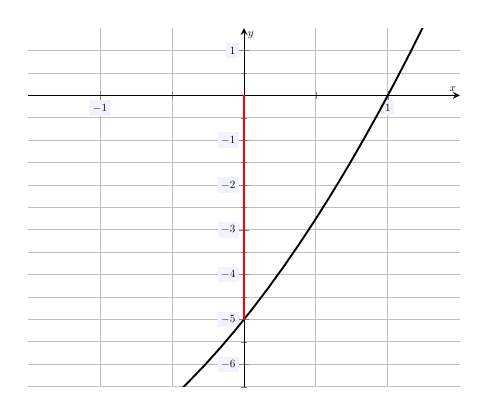
\begin{tikzpicture}[scale=0.8,every node/.style={scale=0.5}]
	\begin{axis}[
	grid=both,
	axis lines=middle,
	ticklabel style={fill=blue!5!white},
	xmin= -1.5, xmax=1.5,
	ymin= -6.5, ymax=1.5,
	xtick={-1,0,...,1},
	ytick={-7,-6,...,1},
	minor x tick num= 1,
	minor y tick num=1,
	xlabel=\(x\),ylabel=\(y\),
	]
	\addplot[domain=-3.5:7.5, samples=100,line width=0.03cm] (x, x^2 + 4*x - 5);
	
	\draw[line width=0.03cm, red, thick] (0,0) -- (0,-5);
	
	\end{axis}
	\end{tikzpicture}
	}
	\]	

\item If $16 \in \im f$, then there is an $x \in \mathbb{R}$ such that $f(x)= 16$. But then\dots
	\[
	\begin{gathered}
	f(x)= 16 \\
	x^2 + 4x - 5= 16 \\
	x^2 + 4x - 21= 0 \\
	(x - 3)(x + 7)= 0 
	\end{gathered}
	\]
But then $x= -7$ or $x= 3$. Observe that $f(-7)= 16$ or $f(3)= 16$. Therefore, $16 \in \im f$. \pspace

\item If $x \in f^{-1}(0)$, then $f(x)= 0$. But then\dots
	\[
	\begin{gathered}
	f(x)= 0 \\
	x^2 + 4x - 5= 0 \\
	(x - 1)(x + 5)= 0 
	\end{gathered}
	\]
But then $x= -5$ or $x= 1$. Observe that $f(-5)= 0$ and $f(1)= 0$. Therefore, $f^{-1}(0)= \{ -5, 1 \}$. \pspace

\item Clearly, the domain and codomain are $\mathbb{R}$, as given in the problem statement. We know the range of $f$ is the image of $f$, i.e. $\im f= \{ f(x) \colon x \in \mathbb{R} \}$. Examining the graph of $f$, we can see that $\im f= f(\mathbb{R})= [-9, \infty)$. We can also see this from the fact that $f(x)= (x + 2)^2 - 9$. 
	\[
	\fbox{
	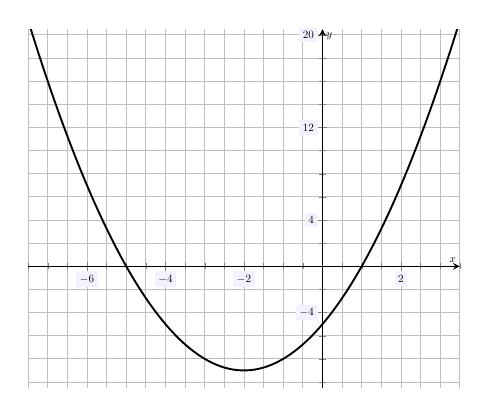
\begin{tikzpicture}[scale=0.8,every node/.style={scale=0.5}]
	\begin{axis}[
	grid=both,
	axis lines=middle,
	ticklabel style={fill=blue!5!white},
	xmin= -7.5, xmax=3.5,
	ymin= -10.5, ymax=20.5,
	xtick={-8,-6,...,4},
	ytick={-12,-4,...,20},
	minor x tick num= 3,
	minor y tick num=3,
	xlabel=\(x\),ylabel=\(y\),
	]
	\addplot[domain=-7.5:3.5, samples=100,line width=0.03cm] (x, x^2 + 4*x - 5);
		
	\end{axis}
	\end{tikzpicture}
	}
	\]
To prove this, suppose that $y \in [-9, \infty)$, choose $x:= \sqrt{9 + y} - 2$, which is well-defined because $y \geq -9$. But then\dots
	\[
	f(x)= (\sqrt{9 + y} - 2)^2 + 4(\sqrt{9 + y} - 2) - 5= (y + 13 - 4 \sqrt{9 + y}) + 4(\sqrt{9 + y} - 2) + 4= y
	\]
So if $y \in [-9, \infty)$, $y \in \im f$. Clearly, if $y < -9$, then $y \notin \im f$: if there were an $x \in \mathbb{R}$ such that $f(x)= y$, then $(x + 2)^2 - 9= y < -9$. This shows that $(x + 2)^2 < 0$, which is impossible. Therefore, $\im f= [-9, \infty)$. Alternatively, we know that $f(-2)= -9$, $\displaystyle \lim_{x \to -\infty} f(x)= \infty$, and $\displaystyle \lim_{x \to \infty} f(x)= \infty$ (because $f$ is an even degree polynomial). We can see that $f(x)= (x + 2)^2 - 9 \geq 0 - 9= -9$. Finally, because $f$ is continuous, by the Intermediate Value Theorem, it must be that $f$ takes on any value in $[-9, c]$ for all $c \in (-9, \infty)$. This again shows that $\im f= [-9, \infty)$. 
\end{enumerate}



\newpage



% Problem 4
\problem{10} Being sure to justify your answer, complete the following:
	\begin{enumerate}[(a)]
	\item Let $f: \mathbb{R} \to \mathbb{R}$ be given by $f(x)= 5 - x^2$. Is $f$ an increasing function? Explain. Is $f$ a decreasing function? Explain. 
	\item Let $g: \mathbb{R} \to \mathbb{R}$ be given by $g(x)= 5x - 8$. Is $g$ a positive function? Explain. Is $g$ a negative function? Explain. 
	\item Let $g$ be as in (b) and define $A= [2, \infty)$ and $B= (-\infty, 0)$. Is $g \big|_A$ a positive function? Explain. Is $g \big|_B$ a negative function? Explain. 
	\item Let $h: \mathbb{R} \to \mathbb{R}$ be given by\dots
		\[
		h(x)= 
		\begin{cases}
		1 - x, & x < 2 \\
		3x + 5, & x \geq 2
		\end{cases}
		\]
	Find the largest possible interval $S \subseteq \mathbb{R}$ such that $h \big|_S$ is a nondecreasing function. Is $h$ monotone on $S$? Is $h$ strictly monotone on $S$?
	\end{enumerate} \pspace

\sol 
\begin{enumerate}[(a)]
\item If $f$ were increasing, then for all $x, y \in \mathbb{R}$ with $x < y$, we would have $f(y) > f(x)$. However, observe that $0 < 1$ but $4= f(1) \not> f(0)= 5$. Therefore, $f$ is not an increasing function. If $f$ is a decreasing function, then for all $x, y \in \mathbb{R}$ with $x < y$, we would have $f(y) < f(x)$. However, observe that $-1 < 0$ but $5= f(0) \not< f(-1)= 4$. Therefore, $f$ is not decreasing. \pspace

\item If $g$ is a positive function, then $g(x) > 0$ for all $x \in \mathbb{R}$. However, observe that $g(0)= -8 \not> 0$. Therefore, $g$ is not a positive function. If $g$ is a negative function, then $g(x) < 0$ for all $x \in \mathbb{R}$. However, observe that $g(2)= 2 \not< 0$. Therefore, $g$ is not a negative function. \pspace

\item From the graph of $g\big|_A$, we can see that $g$ is not a negative function and $g$ is a positive function. 
	\[
	\fbox{
	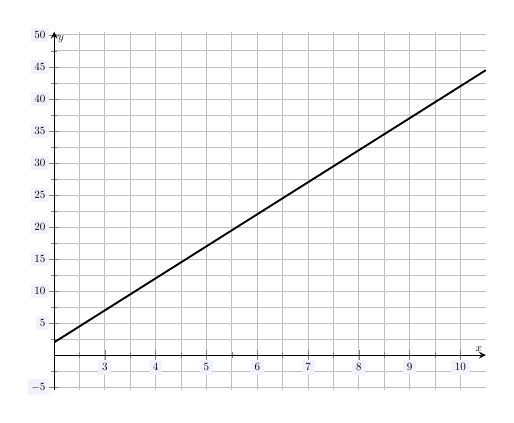
\begin{tikzpicture}[scale=0.8,every node/.style={scale=0.5}]
	\begin{axis}[
	grid=both,
	axis lines=middle,
	ticklabel style={fill=blue!5!white},
	xmin= 2, xmax=10.5,
	ymin= -5.5, ymax=50.5,
	xtick={2,3,...,10},
	ytick={-5,0,...,50},
	minor x tick num= 1,
	minor y tick num=1,
	xlabel=\(x\),ylabel=\(y\),
	]
	\addplot[domain=2:10.5, samples=100,line width=0.03cm] (x, 5*x - 8);
		
	\end{axis}
	\end{tikzpicture}
	}
	\]
To see that $g$ is not negative, observe that $2 \in A$ and $g(2)= 2 \not< 0$. To prove that $g$ is positive, observe that if $x \geq 2$, then\dots
	\[
	\begin{gathered}
	x \geq 2 \\
	5x \geq 10 \\
	5x - 8 \geq 2 \\
	g(x) \geq 2
	\end{gathered}
	\]
But then for $x \geq 2$, $g(x) \geq 2 > 0$. Therefore, $g$ is positive on $A= [2, \infty)$. Now from the graph of $g\big|_B$, we can see that $g$ is negative but not positive. 
	\[
	\fbox{
	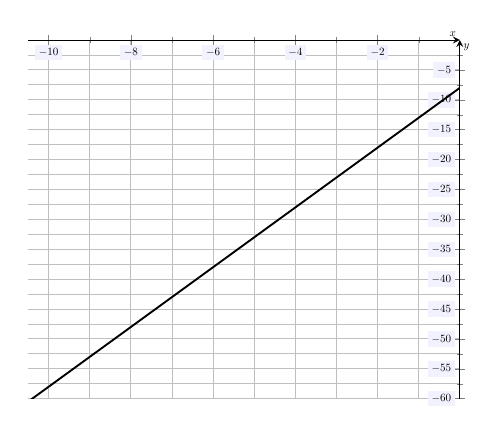
\begin{tikzpicture}[scale=0.8,every node/.style={scale=0.5}]
	\begin{axis}[
	grid=both,
	axis lines=middle,
	ticklabel style={fill=blue!5!white},
	xmin= -10.5, xmax=0,
	ymin= -60, ymax=0,
	xtick={-10,-8,...,0},
	ytick={-60,-55,...,0},
	minor x tick num= 1,
	minor y tick num=1,
	xlabel=\(x\),ylabel=\(y\),
	]
	\addplot[domain=-10.5:0, samples=100,line width=0.03cm] (x, 5*x - 8);
		
	\end{axis}
	\end{tikzpicture}
	}
	\]
To see that $g$ is not positive, observe that $g(0)= -8 \not> 0$. Therefore, $g$ is not positive. To see that $g$ is negative, observe that if $x < 0$, then\dots
	\[
	\begin{gathered}
	x < 0 \\
	5x < 0 \\
	5x - 8 < -8 \\
	g(x) < -8
	\end{gathered}
	\]
But then $g(x) < -8 < 0$. Therefore, $g$ is negative on $B= (-\infty, 0)$. \pspace

\item We first plot $h$, which is shown below.
	\[
	\fbox{
	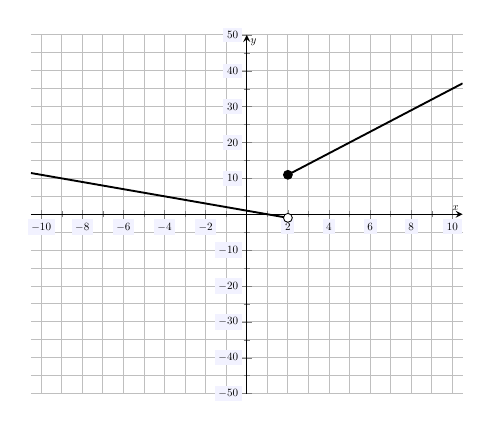
\begin{tikzpicture}[scale=0.8,every node/.style={scale=0.5}]
	\begin{axis}[
	grid=both,
	axis lines=middle,
	ticklabel style={fill=blue!5!white},
	xmin= -10.5, xmax=10.5,
	ymin= -50, ymax=50,
	xtick={-10,-8,...,10},
	ytick={-50,-40,...,50},
	minor x tick num= 1,
	minor y tick num=1,
	xlabel=\(x\),ylabel=\(y\),
	]
	\addplot[domain=-10.5:2, samples=100,line width=0.03cm] (x, 1 - x);
	\addplot[domain=2:10.5, samples=100,line width=0.03cm] (x, 3*x + 5);
	
	\addplot[holdot] coordinates{(2,-1)};
	\addplot[soldot] coordinates{(2,11)};

	\end{axis}
	\end{tikzpicture}
	}
	\] 
Clearly, $h$ is linear on $[2, \infty)$ and $(-\infty, 2)$. On $(-\infty, 2)$, $h \equiv 1 - x$. Because this linear function has negative slope, it is decreasing. In particular, $h$ is not nondecreasing. On $[2, \infty)$, $h \equiv 3x + 5$. Because this linear function has positive slope, it is increasing. In particular, $h$ is then nondecreasing. But then the largest interval on which $h$ is nondecreasing is $S:= [2, \infty)$. Because $h$ is nondecreasing or nonincreasing on $[2, \infty)$, $h$ is monotone on $[2, \infty)$. However, because $h$ is not (strictly) increasing or (strictly) decreasing on $S:= [2, \infty)$, $h$ is not strictly monotone on $S:= [2, \infty)$. 
\end{enumerate}


\end{document}